\documentclass[10pt,conference,compsocconf]{IEEEtran}

\usepackage{hyperref}
\usepackage{amsmath}
\usepackage{graphicx}	% For figure environment
\usepackage{float}
\usepackage{units}
\usepackage{epsfig}
\usepackage{graphicx}
\usepackage{multirow}
\usepackage{cite}
\usepackage{amsmath}
\usepackage{amsfonts}
\usepackage{amssymb}
\usepackage{subfigure}
\usepackage{wrapfig}
\usepackage{multicol}
\def \be {\begin{equation}}
\def \ee {\end{equation}}
\def \bf {\begin{figure}}
\def \ef {\end{figure}}
\graphicspath{{figures/}}


\begin{document}
\title{Deep learning techniques for geometric matching of microscopy images of \textit{C. elegans} brains}

\author{
  Richie Yat-tsai \textsc{Wan}, Pedro \textsc{Bedmar-López},  Longlai \textsc{Qiu}\\
    richie.wan@epfl.ch, pedro.bedmarlopez@epfl.ch, longlai.qiu@epfl.ch\\
  \textit{CS-433 - Ecole Polytechnique Fédérale de Lausanne}\\
  \textit{Project hosted by Prof. Sahand Rahi, LPBS, Institute of Physics, EPFL}
  \\
  \today
}
\maketitle
\begin{abstract}
Deep Learning techniques have been at the forefront of great progress in Computer Vision  tasks, and achieve state of the art on problems such as classification, object segmentation, object detection, among many others. One of the components that make the success of deep learning are convolutional neural networks (CNN). In this report, we propose a model to geometrically match a source image to a target, applied to fluorescence microscopy images of \textit{C. elegans} brains. First, we designed a pipeline to extract 3D images from microscopy data and generate a large training dataset using meaningful data augmentation. Secondly, we adapt a CNN used for geometric matching, initially trained on the Proposal Flow dataset. The adapted network, named \textsc{WormBrain}, instead matches frames of microscopy images of that have undergone deformation, rotation, translation. We added our own architecture for both feature extraction, feature regression, and show that it performs at least as well as the base network. Finally, we align frames extracted from a video.
\end{abstract}

\section{\textbf{Introduction}}
\label{intro}
Computer vision (CV) and pattern recognition (PR) tasks can be applied to datasets pertaining to everyday objects such as CIFAR10, ImageNet. One of the factor in DL techniques' success for CV is the use of CNNs, pioneered with the invention of LeNet5\cite{lecun_gradient-based_1998} to identify handwritten digits and AlexNet \cite{krizhevsky_imagenet_2017} applied to ImageNet among others. DL techniques for CV can also be used in more specialized applications as in the biological or medical field, such as microscopy data. One important techniques to study biological processes is the characterization of cell activity or phenotype by using fluorescent markers. For example, one can label a gene using a fluorescent protein, and use it to track a cell type, or activity such as cell signaling\cite{jiang_specific_2016}. 

Traditionally, the image processing and analysis can be done manually using techniques like thresholding, edge detection, etc. But identifying cells of interest manually over thousands of image frames can prove to be time-consuming, require human intervention and results may be vary depending on the user. On top of that, in biological applications, repeat experiments typically generate large amount of data.

DL can take advantage of this amount of data, whether it is for supervised or unsupervised learning. In CNNs, the network can effectively learn the weights of their kernels in all layers by optimizing a loss over epochs. This yields a network that is tailored to a task such as identifying cells in an image.

In CV, the underlying task is referred to as cell segmentation. Many methods have been developed for automatic cell detection\cite{jiang_geometry-aware_2020,xie_efficient_2018} as well as cell segmentation\cite{dimopoulos_accurate_2014,loewke_automated_2018}. Nevertheless, cell segmentation still poses many challenges\cite{peng_bioimage_2008}, due to different factors such as varying fluorescent intensities, the 3D nature of cells requiring to choose the optimal Z-plane to achieve the best focus, or differences in imaging hardware setups and protocols such as lenses or exposure time.

In the case of this project, the cells in question are not fixed and may move, roll, translate, deform across frames, creating another obstacle for analysis. A subset of neurons are marked with red fluorescent proteins to serve as landmarks, while green nuclear GCaMP has varying intensities with respect to the concentration of intracellular calcium. 
%\vspace{-0.2cm}
%\begin{figure}[h!]
%    \centering
%    \includegraphics[scale = 0.175]{translated_frame.png}
%    \vspace{-0.1cm}
%    \caption{Extracted image frames 137 to 138. The same cells of interest have %shifted and deformed}
%    \label{fig:translated}
%\end{figure}
%\vspace{-0.2cm}

Thus, the aim of this project is to geometrically match and align cells of interests after deformation across frames. To do so, we build upon the work of Rocco et al.\cite{roccoConvolutionalNeuralNetwork2017}, who used a CNN for geometrical matching. The concepts relating to \cite{roccoConvolutionalNeuralNetwork2017} will be expanded upon in section \ref{rocco}. An example of the movement across frames as well as alignment is showcased in figure \ref{fig:demo_worm_brains}.

\vspace{-0.3cm}
%%%%Rocco et al%
\section{\textbf{Basis for our work}}
\label{rocco}
In this section, we expand on the idea behind \cite{roccoConvolutionalNeuralNetwork2017}'s \textsc{cnngeometric} network. Their base implementation can be found at \url{https://github.com/ignacio-rocco/cnngeometric_pytorch}. All figures in this section are taken or adapted from \cite{roccoConvolutionalNeuralNetwork2017}.

\subsection{Architecture}
Their proposed architecture can be separated in three modules and illustrated below in figure \ref{fig:network}.
\begin{itemize}
    \item 1. A CNN Feature Extraction (\textsc{FE}) layer
    \item 2. A CNN Feature Correlation (\textsc{FC}) layer 
    \item 3. A CNN and linear layer for Feature Regression (\textsc{FR})
\end{itemize}

\vspace{-.5cm}
\begin{figure}[h!]
    \centering
    \includegraphics[scale = 0.65]{network_adapted_from_rocco.jpg}
    \vspace{-0.3cm}
    \caption{The architecture proposed by Rocco et al., adapted from their 2017 paper. The FE CNN shares weights for $I_{A}$, $I_{B}$, and outputs the estimated parameters for a given geometric transformation $\hat{\theta}$.}
    \label{fig:network}
\end{figure}

A pair of images goes through the FE layer which extracts relevant features. These are then matched in the FC layer and go through the FR layer. At the end, the output are $\hat{\theta}$, the set of parameters estimated for a given geometric transformation from $I_{A}$ to $I_{B}$. Two geometric transformations have been implemented by the authors, namely affine transformation (\textsc{Aff}) and thin-plate spline transformation (\textsc{TPS}).

\subsubsection{\textsc{Feature Extraction}}
\label{rocco_fe}
From a pair of images $I_{A}$, $I_{B}$, the FE is used to output the feature-maps $f_{A}, f_{B}$. This process is done by a Siamese network\cite{cartwright_siamese_2021, bertinetto_fully-convolutional_2016} that apply the same weights on both inputs. This helps extracting similar features, while removing issues with variation during the first stage across different feature extractors. In their PyTorch implementation, Rocco et al. used either VGG16\cite{simonyan_very_2015} and Resnet101\cite{he_deep_2015} as FEs. The output feature-maps are then L2-normalized on a per-feature basis.

\subsubsection{\textsc{Feature Correlation}}
\label{rocco_fc}
The authors match the feature-maps by computing a correlation map $C_{AB}$. Effectively, each pixel of feature-map is matched to each pixel through a scalar product described in equation \ref{eq:correlation} below, while the result is illustrated in figure \ref{fig:correlation}. 

\vspace{-.2cm}
\begin{equation}
  \label{eq:correlation}
  c_{AB}(i,j,k) = \mathrm{f_B}(i,j)^T \mathrm{f_A}(i_k,j_k)
\end{equation}

\vspace{-0.3cm}
\begin{figure}[h!]
    \centering
    \includegraphics[scale = 0.42]{correlation_layer_adapted.jpg}
    \vspace{-0.3cm}
    \caption{Correlation layer.}
    \label{fig:correlation}
\end{figure}
\vspace{-0.3cm}

\subsubsection{\textsc{Feature Regression}}
\label{rocco_fr}
The correlation map $C_{AB}$ is then L2-normalized and fed through the FR layer. This consists of a simple 2 layers CNN, followed by a single fully connected layer with no activation function to mimic linear regression and estimate the parameters for a given geometric transformation. In the previous layer, dense per-feature matching allows to retain information across large distances from the feature-maps, while local information is retained after passing through a small CNN. The regression layer is regularized through means of BatchNorm as described in figure \ref{fig:base_fr}.

\vspace{-0.2cm}
\begin{figure}[h!]
    \centering
    \includegraphics[scale = 0.335]{base_featureRegression.jpg}
    \vspace{-0.5cm}
    \caption{Feature regression module used by Rocco et al. The output dimension P may be equal to 6 for \textsc{Aff} transformation, or 18 for \textsc{TPS} transformation.}
    \label{fig:base_fr}
\end{figure}


\subsubsection{Two-stage model}
Finally, the authors propose a two-stage model. For a pair of images $I_{A}$, $I_{B}$, they first estimate the parameters for an affine transformation for coarse matching $\hat{\theta}_{Aff}$. Using $\hat{\theta}_{Aff}$, they warp the original image $I_{A}$ and 
they generate another pair from which they estimate the parameters of \textsc{TPS} $\hat{\theta}_{TPS}$ transformation for fine matching. As a result, the total image is first warped using $\hat{\theta}_{Aff}$ followed by $\hat{\theta}_{TPS}$.

\begin{figure}[h!]
    \centering
    \includegraphics[scale = 0.32]{two_stages.jpg}
    \vspace{-0.3cm}
    \caption{Two stages model for coarse then fine alignment. The first stage estimates parameters for \textsc{Aff} transformation, while the second estimates the parameters for \textsc{TPS} transformation.}
    \label{fig:two_stage}
\end{figure}
\vspace{-0.3cm}
%------------------------ PEDRO WRITE HERE
\subsection{Training}
For training, image pairs are generated synthetically: a ${\theta}_{GT}$ ground truth transformation is applied to $I_{A}$, leading to $I_{B}$. These image pairs are used to train the model, a process that consists in reducing the grid loss function error, i.e. minimizing the distance between $\hat{\theta}$ and ${\theta}_{GT}$, the MSE between the transformed grid points and defined in Equation \ref{eq:loss} where $g_i$ is the coordinate
$(x_i, y_i)$ of the uniform grid. 
The parameters are optimized using Adam, and takes about 2 hours to train over 40 epochs using a NVIDIA GeForce RTX 2060.
\begin{equation}
  \label{eq:loss}
  L(\hat{\theta}, \theta_{GT}) = \frac{1}{N} \sum_{i=1}^{N} d(\tau_{\hat{\theta}}(g_i), \tau_{\theta_{GT}}(g_i))^2
\end{equation}



%%%%

\section{\textbf{Data}}
The laboratory we work with has provided us with images of a worm's brain in the form of a video and two .h5 files. These images contain noise and are not perfectly focused, because the worm moves inside the microscope.

\subsection{Data extraction}
The .h5 files are organized as a file system, where there are folders called groups, and within them files called frames. These frames are multidimensional arrays that represent, in our case, 3D images with the following dimensions depending on the file:

\begin{itemize}
    \item {epfl3.h5}: 1715 frames with shape [1,112,112,32], green channel only.
    \item {more\_data.h5}: 575 frames with shape [2,512,512,35], green and red channel.
\end{itemize}

To train the model we will use more\_data.h5, as the images in the other file have too little resolution. Our model works with 2D images with 3 channels, so we transform each frame inside the .h5 file into a 2D image by applying max projection on each channel (see figure \ref{fig:extracted}) and add an empty blue channel.

We use the video frames for testing once the model is trained. Each frame of the video is aligned with the previous frame or a target frame, thus stabilizing it.

\vspace{-0.2cm}
\begin{figure}[h!]
    \centering
    \includegraphics[scale = 0.16]{extracted_frame_0.png}
    \vspace{-0.2cm}
    \caption{\textbf{frame\_0} extracted from the .h5 file. Left shows stacked channels, middle shows the red channel, and right the green channel.}
    \label{fig:extracted}
\end{figure}
%-----------------------------------------------------------
%\vspace{-1.7cm}
\subsection{Data augmentation}
Given the circumvent the small amount of data available for training (572 images), we opted to use data augmentation in a way relevant to our task and generate more training data. The microscopy data we have may sometimes be noisy. The cells of interests are often rotated, translated, and naturally deformed (shear along the X and Y axis). Thus, we wanted to artificially generate data that mimic those conditions.

To do so, we used the library \textsc{imgaug} which can be found at \url{https://imgaug.readthedocs.io/en/latest/}. We've chosen \textsc{imgaug} because of it's ease of use as well as the many random parameters it allows.
We have chosen the following \textbf{methods} for transformation: 

\begin{itemize}
    \item \textbf{ShearX} combined with \textbf{ShearY} for stretching along the X and Y axis, with degrees of shearing sampled uniformly in $(-10,10)^{2}$, once in each dimension.
    \item \textbf{Rotate} with degrees of rotation chosen with equal probability $p=\frac{1}{4}$ in $\{-30,-15, 15, 30\}$
    \item \textbf{PiecewiseAffine} for distorsion, scale sampled in range $(0.01,0.06)$
    \item \textbf{Affine} for translation and zooming, scale sampled uniformly in range $(1.1, 1.2)^{2}$, once for each dimension.
    \item \textbf{AdditiveGaussianNoise}, centered at 0 and amount chosen randomly in scale $(0, \frac{1}{40}\times{255})$
\end{itemize}

Using \textbf{SomeOf}, we randomly choose 2, 3 or 4 transformations with equal probability $p = \frac{1}{3}$ to be applied on a given batch of images. In total, we augment the training images ten-fold, yielding us a total of 5720 of augmented images + 572 original images. From those, we split $80\%$ of it for training set and the remaining $20\%$ for the validation set.


\section{\textbf{Models}}
As we felt the correlation layer is the most important contribution from \cite{roccoConvolutionalNeuralNetwork2017}'s \textsc{cnngeometric model}, we decided to leave that untouched, and rather tune the \textsc{FE} and \textsc{FR}. 

\subsection{Baseline}
As mentioned in section \ref{rocco}, the baseline network uses either VGG16 or Resnet101 with a \textsc{FR} described in \ref{fig:base_fr}.

\subsection{WormBrain}
For our custom architecture from scratch, we've implemented both a FE and two FRs, keeping the feature correlator from \cite{roccoConvolutionalNeuralNetwork2017}. The FE was based on a simple convolutional network, using the same kernel size across layers, with increasing number of channels. To mitigate the effect of vanishing gradients due to the deep architecture and many black pixels from the frames, we opted to use the activation LeakyReLU, as well as BatchNorm2d to regularize. This architecture is shown in figure \ref{fig:wb_fe}.

\vspace{-0.2cm}
\begin{figure}[h!]
    \centering
    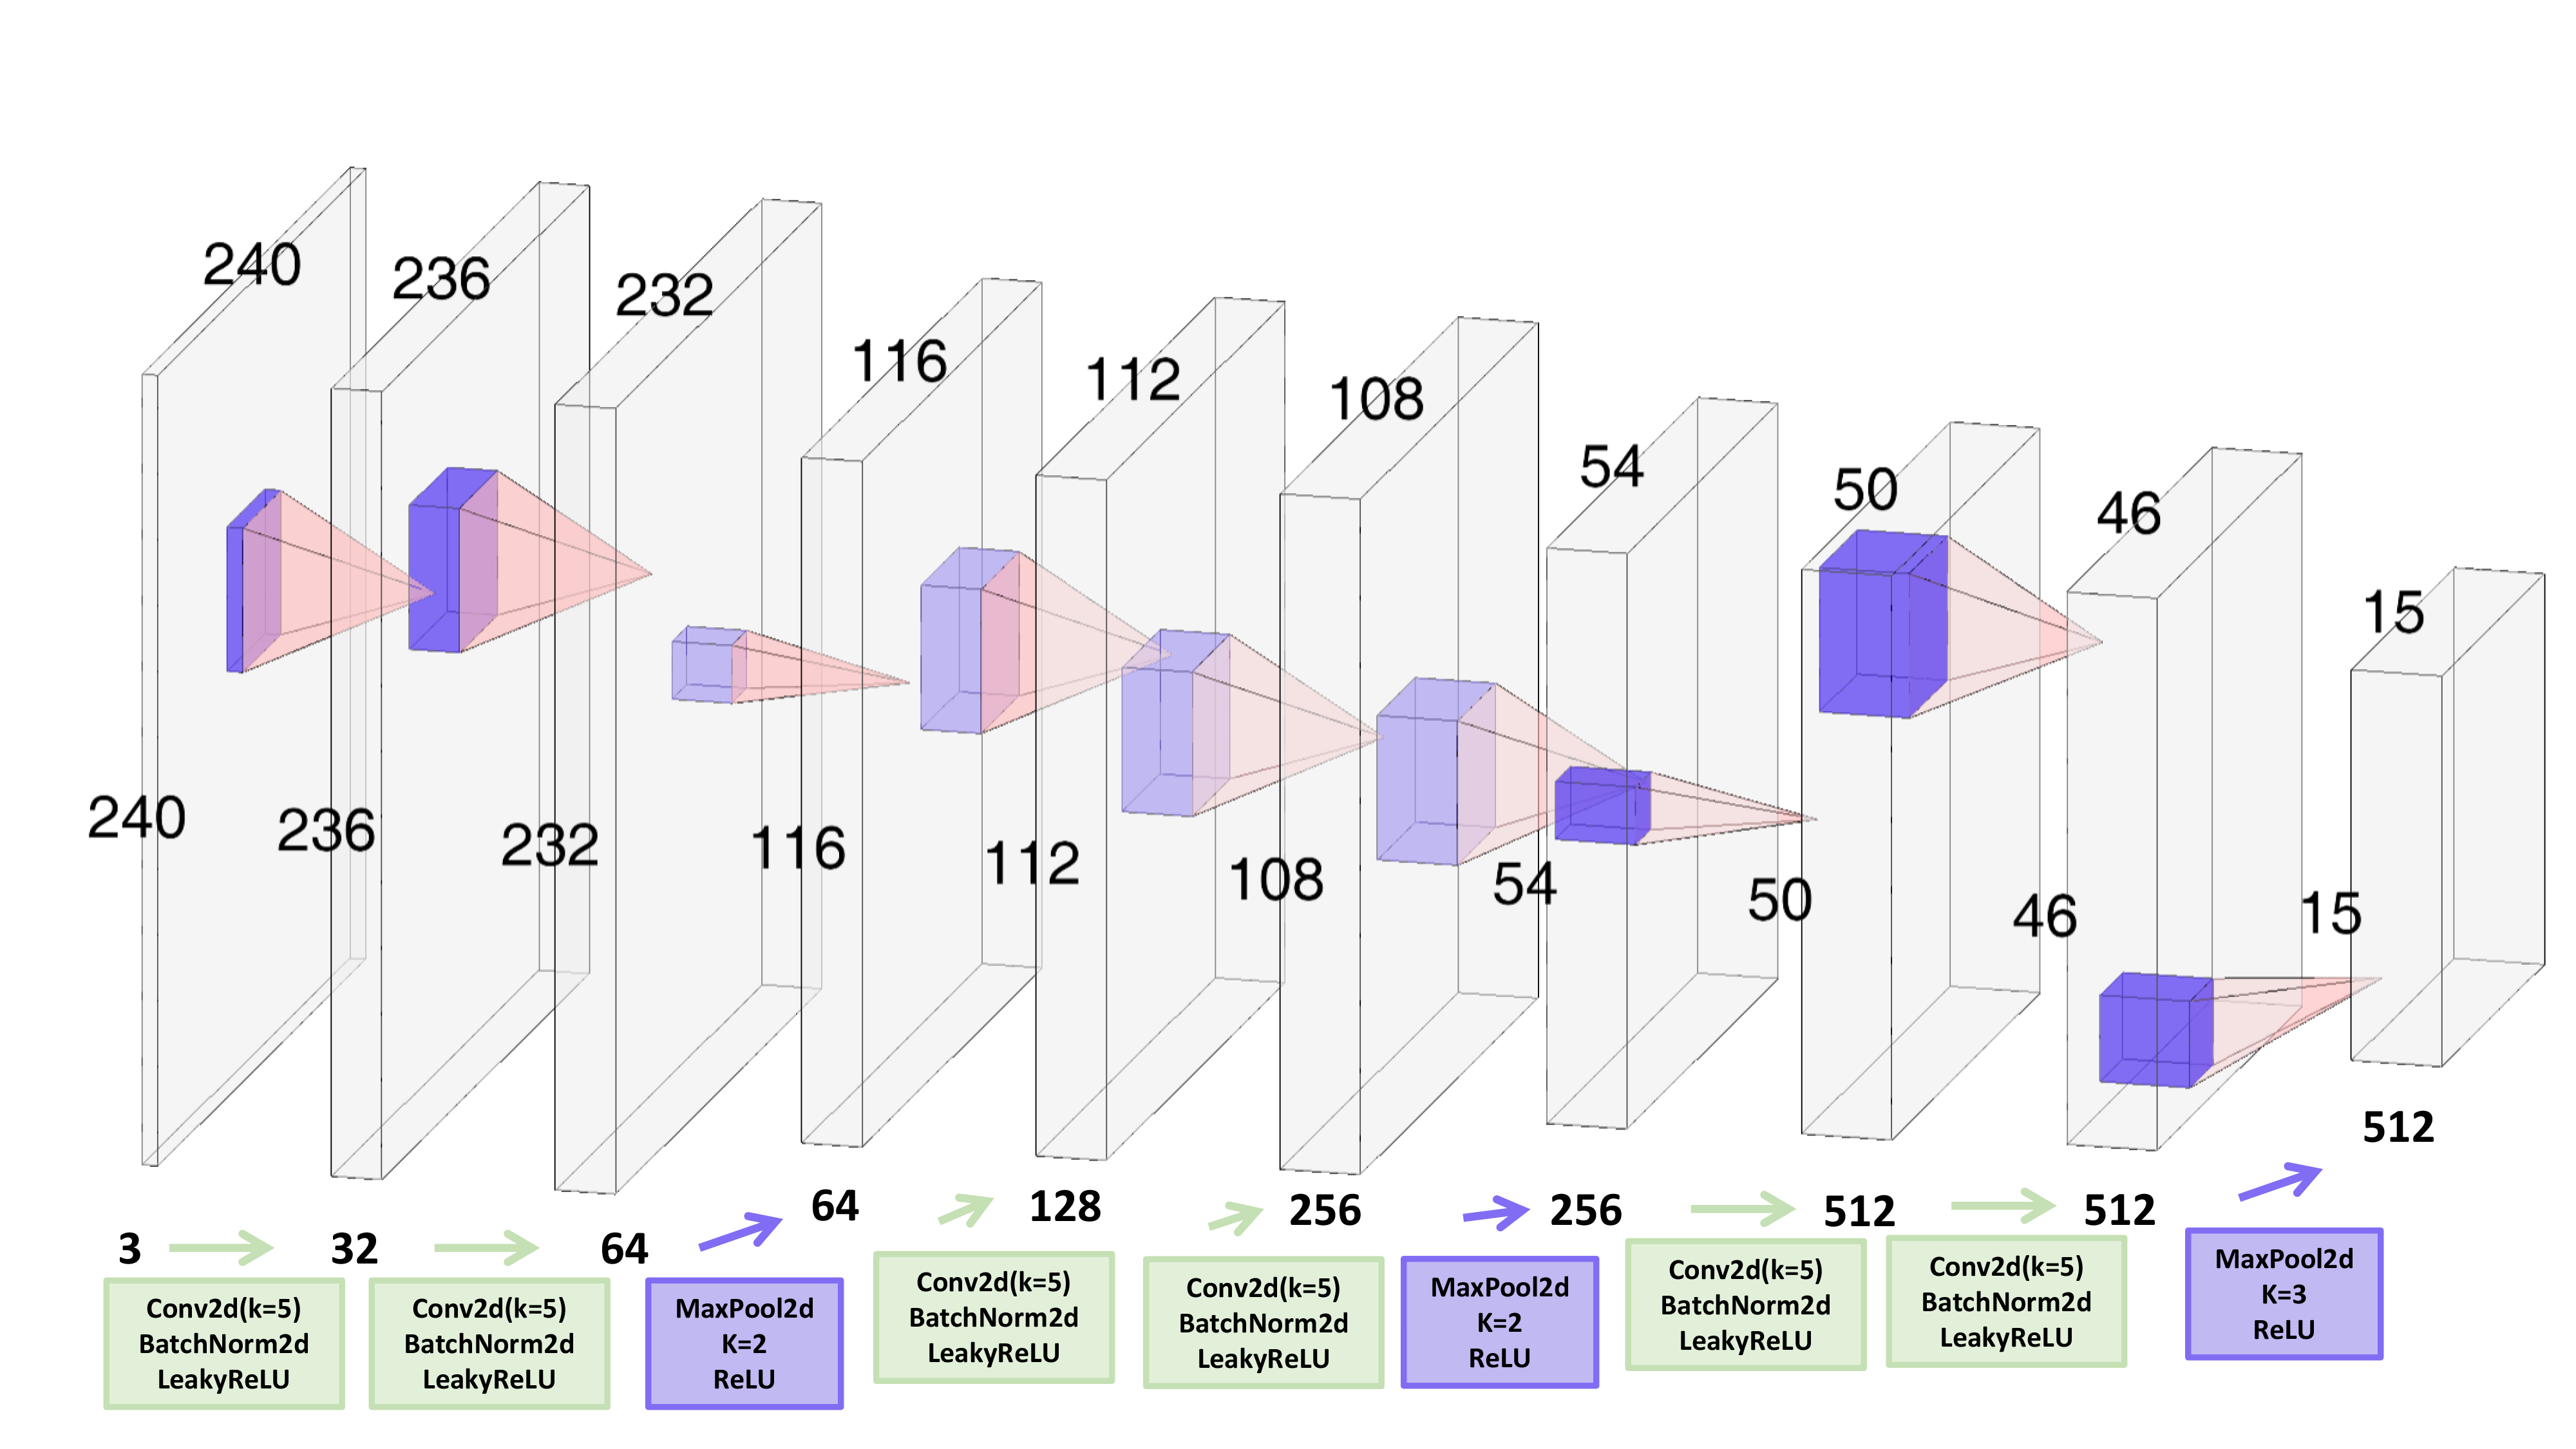
\includegraphics[scale = 0.26]{fext.png}
    \vspace{-0.45cm}
    \caption{\textsc{WormBrain} feature extractor and operations.}
    \label{fig:wb_fe}
\end{figure}
\vspace{-0.2cm}

For the FR, initially, we'd found the prediction layer to be too simple. While the base FR yielded good results for validation loss, when attempting to align images, the results were qualitatively not satisfactory. Instead, we've first tried using a small MLP of 5 layers with number of hidden units decreasing by half in each layer (diagram not shown). Each layer is also regularized using BatchNorm1d and DropOut to make the network better at generalization and encourage the network to learn weights that are more independent of the other hidden units. 

\vspace{-0.2cm}
\begin{figure}[h!]
    \centering
    \includegraphics[scale = 0.19]{simpler_fr.png}
    \vspace{-0.5cm}
    \caption{\textsc{simpler} Feature regression module.}
    \label{fig:simpler_fr}
\end{figure}

This approach was not satisfactory, as shown by figure \ref{fig:tps_loss} and table \ref{tab:validation}. We hypothesized that our model was too deep and did not extract any more useful information through the multiple layers. Using another approach, we decided to first use Softmax as the first activation after the convolutional layers. The idea behind this is that it will normalize all the features to a probability density of range (0,1). In doing so, it mimics a generalization of a multinomial logistic regression where the task is to predict the parameters of the geometric transformation. On top of that, we made the network more shallow while keeping the regularization elements such as BatchNorm and DropOut of 20\%. This yielded the FR shown in figure \ref{fig:simpler_fr}.

\section{\textbf{Results and discussion}}

Given the task, evaluation was strictly done using grid-loss on the validation set, as we do not have a real test-set per se. Probability of Correct Keypoints would have been a good metric, as used in\cite{roccoConvolutionalNeuralNetwork2017}, but would have required manual annotation of many image frames.


\begin{figure}[h!]
    \centering
    \includegraphics[scale = 0.322]{tps_loss.png}
    \vspace{-0.55cm}
    \caption{Training and Validation loss for TPS transformation.}
    \label{fig:tps_loss}
\end{figure}
\vspace{-0.5cm}

\subsection{Training and validation losses} 
As estimation for \textsc{TPS} proved to be more challenging than \textsc{Aff} (Higher grid loss on average, data not shown), all the results we show focus on \textsc{TPS}. Grid-losses on validation sets as well as hyperparameters used during training are summarized in \ref{tab:validation} and evolution of both training and validation loss per epochs are shown in \ref{fig:tps_loss}. Qualitatively, we notice a cyclic behaviour w.r.t. the loss, which could be generated by the CosineAnnealingLR scheduler used in training. The best validation loss reached by our custom architecture (WB+Simpler) manages to achieve results close to the best baseline model (VGG16+Base) with a difference of $9.17\%$, while the loss over epochs appears to be more stable overall. 

\vspace{-0.35cm}
\begin{table}[h!]
  \centering
  \caption{Best validation loss for all models using MSE-Grid loss for Thin-Plate Spline transformation.\\
  \textbf{$\gamma$}:Learning rate, \textbf{Mom} : Momentum used in BatchNorm}
  \vspace{-0.2cm}
  \begin{tabular}{|l||c|c|c|c|c|}
      \hline
      \textbf{FE + FR} & \textbf{$\gamma$} & \textbf{Mom.} & \textbf{Epochs} & \textbf{Best Val. loss}\\ \hline\hline
      VGG16 + Base & 0.001 & 0.9 & 40 & 0.0260 \\ \hline
      Resnet101 + Base & 0.001 & 0.9 & 40 & 0.0428\\ \hline
      WB + Base &  0.00366 & 0.92  & 40 & 0.0294\\ \hline
      WB + Deep &  0.003667 & 0.93 & 40 & 0.0393\\ \hline
      WB + Simpler &  0.005667 & 0.93 & 40 & 0.0285\\ \hline
  \end{tabular}
  \label{tab:validation}
\end{table} 
\vspace{-0.3cm}

\subsection{Alignment}
Qualitatively, we have tried to align images using the base architecture as well as our architecture (WB+Simpler). We have implemented two ways to align frames : the first one requires specifying a target frame, whereas the second one aligns a frame to the previous one. Please e-mail at \url{richie.wan@epfl.ch} for a video demo. It is hard to quantify the actual performance alignment without having the Key Points, but visually, we do notice that our best model (WB+Simpler) tended to yield better results than when we used Resnet101 as a basis.
\vspace{-0.1cm}
\begin{figure}[h!]
    \centering
    \includegraphics[scale = 0.274]{demo_worm_brains.png}
    \vspace{-0.3cm}
    \caption{From left to right : \textsc{src} : source image, \textsc{tgt} : target image, \textsc{aff, tps, aff+tps} : source image after alignment to target image using \textsc{Aff}, \textsc{tps}, \textsc{aff+tps}}
    \label{fig:demo_worm_brains}
\end{figure}
\vspace{-0.25cm}

\section{\textbf{Conclusion}}
In summary, we first introduce a pipeline to extract and use slices of 3D images of dimensions (C,W,H,Z) as training data. Then, we adapt the architecture described in \cite{roccoConvolutionalNeuralNetwork2017}, using a custom architecture and show that we were able to obtain validation grid losses results at least as good as the baseline network of \ref{rocco} re-trained on our dataset. Using our pretrained weights, we can, in a single run, apply the whole pipeline needed for alignment, from data extraction to frames alignment to video generation. For example, our script can take as input either an .h5 file, or a video, or a folder of images, specifying the target frame in the process. It will then save the aligned frames as well as an "aligned.mp4" video.


\subsection{Future steps}
Currently, while every stage of the network is trainable, the loss is only computed with the output of the final stage, with respect to the parameters predicted compared to the ground truth. The gradient flowing backwards all the way to the feature extractor, meaning all three stages of the network train on the loss on outputted parameters. If we have the necessary data, one can improve the training by adding an auxiliary loss at the output of the first stage. For example, if we have cell segmentation maps available (e.g. using another network\cite{dietler_yeaz_2020} to generate them), we can better train the network by jointly training the FE to identify and segment cells, or regressing bounding boxes and computing a loss for the features maps $f_{A}$, $f_{B}$. This way, the network will learn to extract better features with respect to cell segmentation, in the sense that it will better detect useful edges and which part should then be deformed together and aligned from $I_{A}$ to $I_{B}$. 

Beyond the FE, we can also imagine having a FC metric, and a secondary auxiliary loss, for example cosine similarity to be trained jointly. In the end, this yields : 

\vspace{-0.13cm}
\begin{equation}
    \begin{split}
    L_{total} =& \alpha L_{1}(\hat{seg}, seg_{GT})\\
       &+ \beta L_{2}(cor,cos)+\gamma L_{3}(\hat{\theta}, \theta_{GT})
    \end{split}
\end{equation}

Where $\alpha$, $\beta$, $\gamma$ are weights in range $]0,1]$ for the auxiliary loss of each sub-module and the first argument of each loss is the output of that module, and the second argument is the target value on which we compute the loss. Where $L_{3}$ is the grid-loss described in eq.\ref{eq:loss} and functions for $L_{1}$, $L_{2}$ can take various forms, such as MSE loss, CrossEntropyLoss or bounding box regression loss. 

Beyond this, our network currently takes input of shape (3, 240, 240). When using images that are larger, frames are simply resized using bi-linear as implemented by Rocco et al. One key improvement would be to tune the feature extractor, correlator and regressor dimensions to make it even better suited to our datasets, as the frames are of dimension (512,512) and only really contain two color channels and an artificial (empty) blue channel filled with zeros.

\newpage
\bibliographystyle{ieeetr}% nature? IEEE? Elsevier instead
\bibliography{references.bib}%, references_local.bib}
\end{document}

